% IRIDIUM: Provenance-Aware Urban Mobility Platform
% IEEE Transactions on Intelligent Transportation Systems (T-ITS)
% Build: pdflatex -> bibtex -> pdflatex -> pdflatex
\documentclass[journal]{IEEEtran}

% ------------------------------------------------------------------
% Packages
% ------------------------------------------------------------------
\usepackage{amsmath,amssymb,amsfonts}
\usepackage{graphicx}
\graphicspath{{./figures/}}
\usepackage{textcomp}
\usepackage{xcolor}
\usepackage{url}
\usepackage{cite}
\usepackage[utf8]{inputenc}
\usepackage[T1]{fontenc}
\usepackage{hyperref}
\hypersetup{hidelinks}
\usepackage{booktabs}
\usepackage{multirow}
\usepackage{array}
\usepackage{algorithm}
\usepackage{siunitx}
\usepackage{algpseudocode}

% ------------------------------------------------------------------
% Custom commands
% ------------------------------------------------------------------
\newcommand{\R}{\mathbb{R}}
\newcommand{\E}{\mathbb{E}}
\newcommand{\norm}[1]{\left\lVert#1\right\rVert}
\newcommand{\MES}{\mathrm{MES}}
\newcommand{\DS}{\mathtt{status}}

% ------------------------------------------------------------------
% Suppress spurious small-caps-italic substitution warning for all sizes
\DeclareFontShape{T1}{ptm}{m}{scit}
  {<5><6><7><8><9><10><10.95><12><14.4><17.28><20.74><24.88>sub * ptm/m/it}{}

\begin{document}

\title{IRIDIUM: A Provenance-Aware Urban Mobility Platform for
       Digital Twin Assembly, Multimodal Analytics, and Federated
       Learning in Azerbaijani Cities}

% Authors for IEEEtran
\author{
  Olaf~Yunus~Laitinen~Imanov,
  Amina~Sadiqzade,
  Malahat~Ismayilova,
  Aslan~Ibadullayev,
  and~Fidan~Bagirova
\thanks{IRIDIUM Project. This work was conducted as part of an open-source urban mobility platform. Manuscript prepared March 2026.}
}


\maketitle

\begin{abstract}
Urban mobility platforms in data-scarce settings must integrate heterogeneous
real-world feeds while preserving transparent provenance and avoiding
synthetic fallbacks. This paper presents \textit{IRIDIUM}, a
provenance-aware urban mobility platform for Azerbaijani cities, with Baku
as the baseline deployment case. IRIDIUM constructs a request-time digital
twin of the transport network from configured sources, attaches per-source
provenance to every response, and exposes a machine-readable
\texttt{data\_status} field indicating whether returned content is
\texttt{live}, \texttt{recorded}, \texttt{config\_required},
\texttt{permission\_required}, or \texttt{unavailable}. On top of this
twin, the platform defines modular services for congestion forecasting,
multi-objective routing, district-level mobility equity scoring, anomaly
detection, and a federated-learning extension path for privacy-preserving
model training.

The paper formalizes the mobility graph, routing objective,
spatio-temporal forecasting target, equity score, anomaly severity
function, and FedAvg aggregation rule. The current implementation
integrates OpenStreetMap through a PostgreSQL~16/PostGIS~3.4 backend and
ingests live Open-Meteo observations for Baku and Quba; traffic and transit
adapters are registered but remain inactive in the baseline configuration.
Evaluation focuses on three verifiable aspects: API semantics, end-to-end
response latency, and real weather integration. Across $n=50$ loopback
requests per endpoint, median latencies were \SI{2}{ms} for
\texttt{/health}, \SI{45}{ms} for \texttt{/network/graph}, and
\SI{55}{ms} for \texttt{/forecast/congestion}. The weather pipeline
captured a mean Baku--Quba temperature differential of
$\overline{\Delta T} = 2.50 \pm 0.82$\,\textdegree{}C and approximately
16\,mm cumulative precipitation over 72 hours in Baku. Forecasting
accuracy and multimodal-routing benchmarks are intentionally deferred until
traffic histories and transit-feed agreements become available. These
results position IRIDIUM as a transparent baseline architecture for urban
mobility analytics under partial data availability.

\end{abstract}

\begin{IEEEkeywords}
Urban mobility, digital twin, provenance, multimodal routing,
traffic analytics, anomaly detection, federated learning, OpenStreetMap.
\end{IEEEkeywords}

\section*{Notation and Abbreviations}
% ---------------------------------------------------------------
%  Notation and Abbreviations  (IEEE IEEEdescription style)
% ---------------------------------------------------------------

\begin{IEEEdescription}[\IEEEusemathlabelsep\IEEEsetlabelwidth{$\hat{\mathbf{Y}}_{t+1:t+H}$}]

\item[$G=(V,E,W)$] Directed attributed mobility graph.
\item[$V, E$] Node set (junctions, stops, segments) and edge set.
\item[$\mathbf{x}_v$] Node feature vector.
\item[$\mathbf{a}_e$] Edge static attribute vector ($\ell_e$: length, $\tau_e^0$: free-flow time, $c_e$: cost, $\kappa_e$: carbon proxy).
\item[$\mathbf{d}_e(t)$] Edge dynamic state ($s_e$: speed, $\rho_e$: occupancy, $\iota_e$: incident flag).
\item[$\tilde{A}_{uv}$] Distance-weighted adjacency entry.
\item[$\mathbf{X}_t$] Node feature matrix $\in\mathbb{R}^{|V|\times F}$ at time $t$.
\item[$T,\,H$] Lookback window length; forecast horizon.
\item[$\hat{\mathbf{Y}}_{t+1:t+H}$] Multi-step forecast output.
\item[$f_\theta$] Parametric forecasting model (ST-GNN / heuristic).
\item[$K,\,n_k,\,p_k$] FL client count, local dataset size, aggregation weight.
\item[$\theta_k^{(r)}$] Client $k$ parameters after local training in round $r$.
\item[$\varepsilon,\,\delta$] Differential privacy budget parameters.
\item[$J(r)$] Multi-objective route disutility.
\item[$\alpha,\beta,\gamma,\delta$] Routing weight coefficients (time, cost, emissions, penalty).
\item[$\MES_d$] Mobility Equity Score for district $d$.
\item[$\Delta_{\MES}$] Citywide equity gap.
\item[$z_t$] Instantaneous anomaly z-score.
\item[$S_t$] Composite anomaly severity score.
\item[$\tau_S$] Anomaly detection threshold.
\item[$\pi_s$] Source provenance record; $\Pi$: snapshot provenance list.
\item[$\DS$] \texttt{data\_status} field (one of \texttt{live}, \texttt{recorded}, \texttt{config\_required}, \texttt{permission\_required}, \texttt{unavailable}).
\item[$\overline{\Delta T}$] Mean Baku--Quba temperature differential.

\end{IEEEdescription}


\section{Introduction}
\label{sec:intro}
% ---------------------------------------------------------------
%  Section I -- Introduction
% ---------------------------------------------------------------

Urban mobility in rapidly expanding metropolitan areas is shaped by three
interacting structural problems: peak-hour congestion that imposes measurable
economic and environmental costs~\cite{schrank2019tti}, fragmented data
held simultaneously by multiple operators and public agencies, and
regulatory constraints that make centralizing raw personal traces infeasible
in many jurisdictions.
Effective real-time prediction and optimization require integrating
road-network topology, sensor telemetry, transit schedules, atmospheric
conditions, and large-scale event calendars, yet no single operator
typically controls all of these inputs.

Baku, the capital of Azerbaijan and the country's largest urban region,
exemplifies this challenge acutely.
The city has substantially expanded its road network over the past decade
and is investing in an extended metro system and bus-rapid-transit corridors,
yet public, machine-readable GTFS feeds were not available to the authors
during preparation of the baseline release.
Planners and travelers simultaneously need short-horizon congestion forecasts
that can inform signal control and navigation, multimodal journey plans
accounting for current service disruptions, equity-aware accessibility
metrics that identify underserved districts, and incident detection that
distinguishes genuine demand shocks from sensor faults.
In the absence of open data feeds, any deployed platform must communicate
its data-source status explicitly rather than silently degrading or
substituting synthetic data.

\textit{IRIDIUM} is an open-source platform that addresses this operational
and architectural gap through four pillars.

\noindent\textbf{Dynamic digital twin.}
A directed attributed mobility graph $G=(V,E,W)$ is assembled at each
request from all configured real sources.
Nodes represent junctions, road segments, and transit stops; edges carry
mode-specific travel time, monetary cost, carbon proxy, and dynamic state
attributes.
When a source is absent or unconfigured, the assembler returns an empty but
validly typed payload together with an explicit status code, never a
synthetic substitute.

\noindent\textbf{Modular analytics suite.}
A congestion forecaster targets the multi-step prediction
$\hat{\mathbf{Y}}_{t+1:t+H} = f_\theta(\mathbf{X}_{t-T+1:t}, G)$
via a spatio-temporal graph neural network (ST-GNN) extension point with a
heuristic fallback for the pre-model baseline.
A constrained shortest-path router minimizes the weighted functional
$J(r)=\alpha T(r)+\beta C(r)+\gamma E(r)+\delta P(r)$.
A district-level Mobility Equity Score $\MES_d=\sum_m w_m z_{d,m}$
supports spatial justice analysis.
A composite anomaly severity score
$S_t = \lambda_1|z_t|+\lambda_2 e_t+\lambda_3 w_t$ fuses speed deviations
with event and weather signals.

\noindent\textbf{Federated learning pathway.}
Operator nodes train local models on their private datasets and contribute
parameter updates to a central aggregator following the FedAvg rule
$\theta^{(r+1)} = \sum_k p_k\theta_k^{(r)}$~\cite{mcmahan2017fedavg}.
The pathway supports optional $(\varepsilon,\delta)$-differential privacy
noise calibration to protect against gradient inversion
attacks~\cite{kairouz2021advances}.
No federated training experiments are reported in this paper; the FL
component is fully architected and awaits deployment of local training nodes.

\noindent\textbf{Provenance-and-status protocol.}
Every API response carries a machine-readable \texttt{data\_status} tag
and a source provenance list $\Pi = [\pi_{s_1},\ldots,\pi_{s_K}]$
(Eq.~\ref{eq:provenance}).
This design ensures that downstream consumers can always determine whether
a result is grounded in real observations and enables automated data-quality
monitoring as new sources are activated.

\subsection*{Gap Addressed}

Prior work on urban mobility prediction largely relies on either simulated
traffic generation or on proprietary datasets that are unavailable to
independent replication~\cite{pan2019urban,yao2019revisiting,wang2020traffic}.
Platforms built for cities in North America or Western Europe
(METR-LA, PeMS, London TfL) benefit from mature open-data
ecosystems~\cite{li2018dcrnn,wu2019graphwavenet} that do not yet exist
in the South Caucasus region.
IRIDIUM establishes a \textit{real-data stack} in which every source is
documented with acquisition method, license, refresh cadence, and fallback
behavior, enabling honest evaluation under partial data availability and
incremental deployment as operator agreements and feed access become
available.

\subsection*{Contributions}

The primary contributions of this paper are as follows.
\begin{enumerate}
  \item A precise, self-consistent mathematical formalization of the
        mobility graph, the multi-objective routing functional,
        the ST-GNN forecasting target, the Mobility Equity Score,
        the composite anomaly severity score, and the FedAvg aggregation
        step, each consistent with the implemented codebase
        (Section~\ref{sec:formulation}).
  \item A layered system architecture specification that makes the
        provenance-and-status protocol a first-class citizen of
        every API response, supported by a formal description of the
        five-layer platform design and the state-assembly algorithm
        (Tables~\ref{tab:layers}--\ref{tab:pipeline},
        Section~\ref{sec:formulation}).
  \item A real-data ingestion stack covering OpenStreetMap/PostGIS,
        Open-Meteo, and a provider-agnostic traffic and transit
        abstraction layer with quantified data-access status for all
        eight registered sources
        (Section~\ref{sec:data}).
  \item A baseline evaluation covering API semantic correctness,
        end-to-end response latency with fitted log-normal parameters,
        and a real 72-hour weather time-series integration for Baku
        and Quba, including a quantification of the persistent
        inter-city temperature differential
        (Sections~\ref{sec:setup}--\ref{sec:results}).
  \item A candid, mathematically grounded accounting of all unresolved
        operator dependencies, data-access gaps, and evaluation
        limitations (Section~\ref{sec:limitations}).
\end{enumerate}

The IRIDIUM codebase, configuration files, and dataset documentation
are publicly available at
\url{https://github.com/iridium-oss/iridium}.

The remainder of this paper is organized as follows.
Section~\ref{sec:related} reviews related work.
Section~\ref{sec:formulation} formalizes the system model.
Section~\ref{sec:data} describes the data sources.
Section~\ref{sec:methods} details the implemented pipeline.
Section~\ref{sec:setup} explains the experimental setup.
Section~\ref{sec:results} presents results.
Section~\ref{sec:discussion} discusses implications.
Section~\ref{sec:limitations} addresses limitations, ethics, and privacy.
Section~\ref{sec:conclusion} concludes.


\section{Related Work}
\label{sec:related}
% ---------------------------------------------------------------
%  Section II -- Related Work
% ---------------------------------------------------------------

\subsection{Federated Learning and Privacy-Aware Mobility}

Federated learning~\cite{mcmahan2017fedavg} enables model training across
distributed data holders without transmitting raw records to a central server.
McMahan et al.\ introduced FedAvg, in which clients execute $\tau$ local
stochastic gradient descent steps and the server aggregates parameter
updates weighted by local sample size; this mechanism is the conceptual
basis for the IRIDIUM FL pathway.
Li et al.\ \cite{li2020fedprox} showed that heterogeneous client drift can
be mitigated by adding a proximal regularization term
$\mu/2\,\norm{\theta - \theta^{(r)}}^2$ to each client's objective.
Li et al.\ \cite{li2020fedavg_convergence} established convergence bounds
for FedAvg under non-IID data distributions, which is a practically
critical condition when mobility data are partitioned by operator or
district: for non-convex objectives, FedAvg converges at rate
$\mathcal{O}(1/\sqrt{TK})$ under bounded gradient variance.
Kairouz et al.\ \cite{kairouz2021advances} provide a comprehensive survey
covering Byzantine robustness, communication compression, and differential
privacy, all relevant to a multi-operator Azerbaijani deployment.
Lim et al.\ \cite{lim2020federated_edge} survey FL in mobile edge networks,
highlighting that latency constraints and device heterogeneity impose strict
bounds on communication rounds.
IRIDIUM positions its FL component as a fully specified architectural
extension point awaiting local training node deployment.

\subsection{Spatio-Temporal Traffic Forecasting}

Short-horizon traffic forecasting has been substantially advanced by
graph-structured deep learning.
Li et al.\ \cite{li2018dcrnn} proposed the diffusion convolutional recurrent
network (DCRNN), which models traffic as a bidirectional diffusion process
on the road graph and outperforms recurrent baselines on METR-LA and
PeMS-BAY by leveraging spatial correlations.
Yu et al.\ \cite{yu2018stgcn} introduced spatio-temporal graph convolutional
networks (ST-GCN) using purely convolutional temporal operations for
faster training.
Graph WaveNet~\cite{wu2019graphwavenet} extended the framework with
adaptive, self-learned adjacency matrices that capture non-local dependencies
absent from static proximity graphs.
Guo et al.\ \cite{guo2019astgcn} added attention mechanisms over both spatial
and temporal dimensions, yielding attention-based ST-GCN (ASTGCN) with
improved interpretability on PEMS datasets.
Jiang and Luo~\cite{jiang2022gnn_survey} survey graph neural networks for
traffic forecasting comprehensively.
The ST-GNN extension point in IRIDIUM follows Eq.~(\ref{eq:forecast})
and Eq.~(\ref{eq:gcn}); a heuristic baseline is active until a historical
observation store of sufficient length is assembled.

\subsection{Urban Digital Twins and Transport Platforms}

The concept of a city-scale digital twin is gaining traction in research
and practice.
Ferre-Bigorra et al.\ \cite{ferrebigorra2022urban_digital_twins} analyze
adoption barriers including data governance and interoperability, which
directly motivate the provenance-and-status design of IRIDIUM.
Wan et al.\ \cite{wan2024urban_modelling_to_city_digital_twins} trace the
transition from offline urban modelling to continuously updated digital
twins with live sensor fusion.
Weil et al.\ \cite{weil2023urban_digital_twin_challenges} systematically
review challenges and sustainability requirements.
Nag et al.\ \cite{nag2025digital_twins_transport_planning} and
Yan et al.\ \cite{yan2023digital_twin_transport_infra} survey digital
twin applications in transport planning and infrastructure management.
A key distinction of IRIDIUM is that the twin is assembled dynamically from
real configured sources at every request, rather than frozen at a
batch-update boundary.

\subsection{Multimodal Routing and Accessibility}

Delling et al.\ \cite{delling2015raptor} introduced the RAPTOR algorithm
for round-based public-transit routing, achieving practical query times
on city-scale networks through range-based Dijkstra extensions.
Pfertner et al.\ \cite{pfertner2023multimodal_accessibility} describe an
open-source methodology for multimodal accessibility analysis using
OpenTripPlanner and PostGIS.
Graff et al.\ \cite{graff2024nomad} construct a routable, multi-cost,
time-dependent network suitable for combined road and transit optimization.
Gil~\cite{gil2015multimodal_osm_accessibility} builds a multimodal network
directly from OpenStreetMap for sustainable urban accessibility analysis.
IRIDIUM generalizes the routing objective to the weighted sum in
Eq.~(\ref{eq:routing}), covering travel time, monetary cost, carbon
emissions, and transfer penalties; full OpenTripPlanner integration is
deferred until GTFS feeds are available.

\subsection{Mobility Equity Measurement}

Karner et al.\ \cite{karner2025transportation_equity} discuss advances and
methodological pitfalls in measuring transportation equity, noting that
composite indices must account for indicator selection bias and distributional
assumptions.
Guo et al.\ \cite{guo2020transportation_equity_overview} provide a systematic
overview spanning accessibility, emissions, and safety dimensions.
Martens et al.\ \cite{martens2019measuring_transport_equity_metrics} and
Lucas et al.\ \cite{lucas2019measuring_transport_equity_book} define
key components and metrics for transport equity measurement.
The IRIDIUM Mobility Equity Score (Eq.~\ref{eq:mes}) is a district-level
composite of normalized indicators reported as a derived analytic index and
not as an official government statistic.

\subsection{Anomaly Detection in Transportation}

Pramanik et al.\ \cite{pramanik2022traffic_anomaly_video} employ
spatio-temporal rough-fuzzy granulation for video-based anomaly detection
in road surveillance.
Hassan et al.\ \cite{hassan2019spatiotemporal_anomaly_its} address
spatio-temporal detection in intelligent transportation systems using
statistical and machine-learning methods.
IRIDIUM adopts a rule-based composite severity score
(Eq.~\ref{eq:anomaly_severity}) that fuses rolling z-scores over speed
deviations with event-proximity and adverse-weather signals.

\subsection{Comparison with Related Systems}

Table~\ref{tab:related_systems} positions IRIDIUM against representative
urban mobility and traffic forecasting platforms across six dimensions.
The key differentiators of IRIDIUM are: (i) the strict no-synthetic-substitution
policy enforced through a machine-readable status protocol; (ii) the
FL architectural pathway for multi-operator privacy preservation; and
(iii) the explicit targeting of a data-scarce, data-governance-constrained
environment in the South Caucasus.

\begin{table*}[t]
\caption{Comparison of IRIDIUM with representative urban mobility and traffic
         forecasting platforms. Checkmarks indicate supported or planned
         capabilities; dashes indicate that the property is absent or
         not applicable. \textit{Arch.} denotes an architected capability
         not yet evaluated experimentally.}
\label{tab:related_systems}
\centering
\renewcommand{\arraystretch}{1.20}
\begin{tabular}{@{}lcccccccc@{}}
\toprule
\textbf{Platform} &
\textbf{RT} &
\textbf{FL} &
\textbf{Prov.} &
\textbf{OSS} &
\textbf{Multi.} &
\textbf{Equity} &
\textbf{Region} &
\textbf{Open data} \\
\midrule
IRIDIUM (this work)
  & \checkmark & \checkmark$^*$ & \checkmark & \checkmark
  & \checkmark & \checkmark & AZ & Yes \\
DCRNN~\cite{li2018dcrnn}
  & \checkmark & -- & -- & \checkmark
  & -- & -- & US & Curated \\
Graph WaveNet~\cite{wu2019graphwavenet}
  & \checkmark & -- & -- & \checkmark
  & -- & -- & US & Curated \\
ASTGCN~\cite{guo2019astgcn}
  & \checkmark & -- & -- & \checkmark
  & -- & -- & US & Curated \\
Urban DT~\cite{nag2025digital_twins_transport_planning}
  & Varies & -- & Partial & Varies
  & Varies & -- & Various & Varies \\
OTP / Valhalla
  & Partial & -- & -- & \checkmark
  & \checkmark & -- & Global & GTFS/OSM \\
FedMob~\cite{lim2020federated_edge}
  & \checkmark & \checkmark & -- & --
  & -- & -- & Various & Private \\
\bottomrule
\multicolumn{9}{@{}l@{}}{\footnotesize RT: real-time; FL: federated learning ($^*$arch.); Prov.: provenance; OSS: open-source; Multi.: multimodal; AZ: Azerbaijan.}
\end{tabular}
\end{table*}

\subsection{Data Standards and Open Geospatial Infrastructure}

GTFS~\cite{gtfs_overview} and GTFS Realtime~\cite{gtfs_realtime_overview}
define the transit data standards that IRIDIUM targets for integration.
OpenStreetMap provides the base road-network topology; Klinkhardt et al.\
\cite{klinkhardt2023osm_poi_quality} assess OSM point-of-interest quality,
while Moradi et al.\ \cite{moradi2022osm_road_quality} analyze road-network
quality indicators relevant to routing accuracy.
IRIDIUM fetches the Geofabrik Azerbaijan extract, stores the SHA-256 file
checksum in a manifest table, and records full provenance for
reproducibility.


\section{System Architecture and Problem Formulation}
\label{sec:formulation}
% ---------------------------------------------------------------
%  Section III -- System Architecture and Problem Formulation
% ---------------------------------------------------------------

The IRIDIUM platform is organized into five functional layers, each with a
defined interface boundary and a set of registered data-source adapters.
Table~\ref{tab:layers} enumerates all layers, their constituent components,
the technology stack at the time of publication, and their deployment
readiness.
Table~\ref{tab:pipeline} describes the state-assembly pipeline that
implements the merge-only provenance policy.
These two tables replace a block-diagram representation deliberately: by
enumerating every component together with its runtime role and readiness
label, the architecture description becomes auditable and implementation
proximate, consistent with the provenance-first design philosophy of
IRIDIUM.

\begin{table*}[t]
\caption{IRIDIUM five-layer platform architecture. Each component is listed
         with its technology stack, deployment readiness, and activation
         state in the current release. ``Arch.'' denotes an architected
         component not yet operationally deployed.}
\label{tab:layers}
\centering
\renewcommand{\arraystretch}{1.20}
\begin{tabular}{@{}llllcc@{}}
\toprule
\textbf{Layer} &
\textbf{Component} &
\textbf{Technology} &
\textbf{Function} &
\textbf{Readiness} &
\textbf{Active} \\
\midrule
\multirow{7}{*}{External Sources}
  & Road network (OSM)          & Geofabrik PBF / HTTP & Topology data       & live              & Yes \\
  & Weather (Open-Meteo)        & REST / JSON          & Atmospheric data    & live              & Yes \\
  & Traffic (TomTom Flow)       & Licensed REST        & Speed telemetry     & config.\ req.     & No  \\
  & Transit (Baku Metro)        & GTFS / Agreement     & Schedule data       & perm.\ req.       & No  \\
  & Transit (BakuBus)           & GTFS / Agreement     & Schedule data       & perm.\ req.       & No  \\
  & Telemetry (Traccar)         & Consent-based GPS    & Crowd-sourced speed & not impl.         & No  \\
  & Events (iTicket)            & ToS review           & Event calendar      & not impl.         & No  \\
\midrule
\multirow{2}{*}{Ingestion \& Validation}
  & Schema validator            & Pydantic v2 / Python & Type-safe parsing   & live              & Yes \\
  & Provenance recorder         & Custom Python        & Lineage tracking    & live              & Yes \\
\midrule
\multirow{2}{*}{Digital Twin Assembler}
  & Graph builder               & PostgreSQL~16/PostGIS~3.4 & Topology merge & live              & Yes \\
  & State aggregator            & Python / NetworkX   & Dynamic state merge & live (partial)    & Yes \\
\midrule
\multirow{5}{*}{Analytics}
  & Congestion forecaster       & ST-GNN / heuristic  & Speed prediction    & heuristic only    & Partial \\
  & Multi-objective router      & Dijkstra / OTP (plan.) & Path optimization & baseline only     & Partial \\
  & Equity scorer               & NumPy               & $\MES_d$ computation & live             & Yes \\
  & Anomaly detector            & SciPy / Python      & Severity scoring    & live              & Yes \\
  & FL aggregator               & Flower (planned)    & FedAvg gradient agg.& arch.\ only       & No  \\
\midrule
\multirow{2}{*}{REST API}
  & API server                  & FastAPI / uvicorn~0.29 & HTTP interface  & live              & Yes \\
  & Status propagator           & Custom Python       & $\Pi$ attachment    & live              & Yes \\
\bottomrule
\end{tabular}
\end{table*}

\begin{table*}[t]
\caption{Digital twin state-assembly pipeline stages. Each stage produces a
         partial snapshot merged into the global graph $G$.
         Data-status labels propagate from acquisition through all
         downstream stages.}
\label{tab:pipeline}
\centering
\renewcommand{\arraystretch}{1.20}
\begin{tabular}{@{}clll@{}}
\toprule
\textbf{Stage} & \textbf{Operation} & \textbf{Input} & \textbf{Output} \\
\midrule
1 & Fetch            & Source adapter  & Raw bytes or HTTP response \\
2 & Validate         & Raw payload     & Typed Pydantic model \\
3 & Normalize        & Pydantic model  & Internal snapshot object \\
4 & Attach provenance& Snapshot + meta & $\pi_s$ record \\
5 & Merge into $G$   & Partial graph   & Updated $G$ (if \texttt{live} or \texttt{recorded}) \\
6 & Aggregate status & $\{\DS_s\}$     & $\DS_{\mathrm{global}}$ via Eq.~(\ref{eq:global_status}) \\
7 & Emit snapshot    & $G,\,\Pi$       & JSON API response \\
\bottomrule
\end{tabular}
\end{table*}

\subsection{Mobility Graph}

Let $G = (V, E, W)$ be a directed, attributed, multi-modal graph.
The node set
\begin{equation}
  V = V_\mathrm{seg} \cup V_\mathrm{jct} \cup V_\mathrm{stop}
\end{equation}
partitions into road segments, junctions, and transit stops.
Each node $v \in V$ carries a feature vector
\begin{equation}
  \mathbf{x}_v = [\text{type},\; \text{lat},\; \text{lon},\;
                  \text{mode}]^\top \in \mathcal{X}_v,
\end{equation}
where $\text{mode} \in \{\text{road, bus, metro, walking, cycling}\}$.
Each directed edge $e = (u,v) \in E$ carries a static attribute vector
\begin{equation}
  \mathbf{a}_e = [\ell_e,\; \tau_e^0,\; c_e,\; \kappa_e]^\top,
\end{equation}
where $\ell_e$ is edge length (m), $\tau_e^0$ is free-flow travel time (s),
$c_e$ is a generalized monetary cost (AZN), and $\kappa_e$ is a carbon
proxy (g CO$_2$-eq).
The optional dynamic state vector
\begin{equation}
  \mathbf{d}_e(t) = [s_e(t),\; \rho_e(t),\; \iota_e(t)]^\top
\end{equation}
carries current speed $s_e(t)$ (m\,s$^{-1}$), occupancy $\rho_e(t) \in [0,1]$,
and incident flag $\iota_e(t) \in \{0,1\}$.
The graph is assembled exclusively from configured real sources.
When no network import has been executed, $V = E = \emptyset$ and the
assembler returns $\DS = \texttt{config\_required}$.

The adjacency matrix $\mathbf{A} \in \{0,1\}^{|V|\times|V|}$ has
$A_{uv} = 1$ if $(u,v) \in E$.
A distance-weighted variant
\begin{equation}
  \tilde{A}_{uv} = \exp\!\left(-\frac{\ell_{uv}^2}{\sigma_\ell^2}\right)
  \cdot \mathbf{1}[(u,v)\in E]
  \label{eq:adj_weighted}
\end{equation}
with bandwidth $\sigma_\ell$ is used by the ST-GNN layer to encode
proximity-based spatial influence.

\subsection{Forecasting Formulation}

Let $\mathbf{X}_t \in \R^{|V| \times F}$ denote the node feature matrix
at time $t$ over $F$ features (speed, occupancy, weather conditions).
Given a lookback window of length $T$, the multi-step forecasting target is
\begin{equation}
  \hat{\mathbf{Y}}_{t+1:t+H} = f_\theta\!\left(
    \mathbf{X}_{t-T+1:t},\; G\right),
  \label{eq:forecast}
\end{equation}
where $H$ is the forecast horizon and $f_\theta$ is the parametric model.
Standard regression metrics for the held-out evaluation are
\begin{align}
  \mathrm{MAE}  &= \frac{1}{nH}\sum_{i=1}^{n}\sum_{h=1}^{H}
                   \left|y_{i,h} - \hat{y}_{i,h}\right|,
                   \label{eq:mae} \\
  \mathrm{RMSE} &= \sqrt{\frac{1}{nH}\sum_{i=1}^{n}\sum_{h=1}^{H}
                   \left(y_{i,h} - \hat{y}_{i,h}\right)^2},
                   \label{eq:rmse} \\
  \mathrm{MAPE} &= \frac{100\%}{nH}\sum_{i=1}^{n}\sum_{h=1}^{H}
                   \left|\frac{y_{i,h} - \hat{y}_{i,h}}{y_{i,h}}\right|.
                   \label{eq:mape}
\end{align}
The graph convolution step in a single ST-GNN layer reads
\begin{equation}
  \mathbf{H}^{(\ell+1)} = \sigma\!\left(
    \tilde{\mathbf{D}}^{-\tfrac{1}{2}}\tilde{\mathbf{A}}
    \tilde{\mathbf{D}}^{-\tfrac{1}{2}}\,
    \mathbf{H}^{(\ell)}\,\mathbf{\Theta}^{(\ell)}\right),
  \label{eq:gcn}
\end{equation}
where $\tilde{\mathbf{A}} = \mathbf{A} + \mathbf{I}$,
$\tilde{\mathbf{D}}$ is its degree matrix,
$\mathbf{\Theta}^{(\ell)}$ is the trainable weight matrix for layer $\ell$,
and $\sigma(\cdot)$ is a nonlinear activation (ReLU in the baseline
configuration).
The temporal dimension is handled by a gated recurrent unit (GRU) or
dilated causal convolution applied over the sequence
$\mathbf{H}^{(\ell)}_{t-T+1:t}$.

\subsection{Federated Aggregation (Architectural)}

Let there be $K$ client nodes, each holding a local dataset $\mathcal{D}_k$
of size $n_k = |\mathcal{D}_k|$.
The global FL objective is
\begin{equation}
  \min_{\theta}\; \sum_{k=1}^{K} p_k\, \mathcal{L}_k(\theta),
  \quad p_k = \frac{n_k}{\sum_{j=1}^{K} n_j},
  \label{eq:fl_obj}
\end{equation}
where
$\mathcal{L}_k(\theta) = \E_{(\mathbf{x},y)\sim\mathcal{D}_k}
[\ell(f_\theta(\mathbf{x}), y)]$.
The FedAvg global update after communication round $r$ is
\begin{equation}
  \theta^{(r+1)} = \sum_{k=1}^{K} p_k\, \theta_k^{(r)},
  \label{eq:fedavg}
\end{equation}
where $\theta_k^{(r)}$ is the parameter vector of client $k$ after $\tau$
local gradient steps.
Under the non-IID convergence result of Li et al.\
\cite{li2020fedavg_convergence}, the expected gradient norm satisfies
\begin{equation}
  \frac{1}{R}\sum_{r=0}^{R-1}
  \E\!\left[\norm{\nabla \mathcal{L}(\theta^{(r)})}^2\right]
  \leq
  \frac{2(\mathcal{L}(\theta^{(0)}) - \mathcal{L}^*)}
       {\eta\sqrt{RTK}}
  + \mathcal{O}\!\left(\frac{\eta\Gamma^2}{K}\right),
  \label{eq:fl_convergence}
\end{equation}
where $R$ is the total number of communication rounds, $\eta$ is the
learning rate, and $\Gamma^2$ quantifies the non-IID degree (gradient
divergence across clients).
The communication overhead per round scales as
$\mathcal{O}(K \cdot |\theta|)$ bits for uncompressed transfers, reducible
to $\mathcal{O}(K \cdot d \log b)$ for $d$-dimensional quantized updates
with $b$ bits per coordinate~\cite{kairouz2021advances}.

\subsection{Routing Objective}

A route $r = (e_1, e_2, \ldots, e_L)$ is an ordered sequence of edges
in $G$.
The scalar disutility to minimize is
\begin{equation}
  J(r) = \alpha\, T(r) + \beta\, C(r) + \gamma\, E(r) + \delta\, P(r),
  \label{eq:routing}
\end{equation}
where:
$T(r) = \sum_{e \in r} \tau_e(t)$ is realized travel time (s);
$C(r) = \sum_{e \in r} c_e$ is generalized monetary cost (AZN);
$E(r) = \sum_{e \in r} \kappa_e \cdot \ell_e$ is the emissions proxy
(g CO$_2$-eq); $P(r)$ is a mode-transfer or accessibility penalty;
$\alpha, \beta, \gamma, \delta \geq 0$ are user-configurable weights with
$\alpha + \beta + \gamma + \delta > 0$.
The feasibility constraint enforces a maximum journey time $T_{\max}$:
\begin{equation}
  \sum_{e \in r} \tau_e(t) \leq T_{\max},
  \quad r \in \mathcal{R}(o, d),
  \label{eq:routing_constraint}
\end{equation}
where $\mathcal{R}(o,d)$ is the set of all paths from origin $o$ to
destination $d$ in $G$.
When dynamic edge state $\mathbf{d}_e(t)$ is available from a configured
traffic provider, the realized travel time is
$\tau_e(t) = \ell_e / s_e(t)$; otherwise,
$\tau_e(t) = \tau_e^0$.
The computational complexity of Dijkstra's algorithm over $G$ is
$\mathcal{O}((|V|+|E|)\log|V|)$ with a Fibonacci heap priority queue,
which is tractable for Baku's road graph ($|V| \approx 10^5$,
$|E| \approx 2.5 \times 10^5$ from the OSM extract).

\subsection{Mobility Equity Score}

For district $d \in \mathcal{D}$ and accessibility indicator
$m \in \{1, \ldots, M\}$, let $x_{d,m}$ denote the raw indicator value
with empirical mean $\mu_m$ and standard deviation $\sigma_m$ over all
$|\mathcal{D}|$ districts.
The normalized indicator is
\begin{equation}
  z_{d,m} =
  \begin{cases}
    (x_{d,m} - \mu_m)\,/\,\sigma_m & \text{if } \sigma_m > 0, \\
    0 & \text{otherwise,}
  \end{cases}
  \label{eq:zscore_district}
\end{equation}
and the Mobility Equity Score for district $d$ is
\begin{equation}
  \MES_d = \sum_{m=1}^{M} w_m\, z_{d,m},
  \quad \text{s.t.}\;\sum_{m=1}^{M} w_m = 1,\; w_m \geq 0.
  \label{eq:mes}
\end{equation}
The citywide equity gap is
\begin{equation}
  \Delta_{\MES} = \max_{d \in \mathcal{D}} \MES_d
                - \min_{d \in \mathcal{D}} \MES_d,
  \label{eq:equity_gap}
\end{equation}
a scalar summary of spatial inequality in mobility access.
The variance of $\MES_d$ across districts,
\begin{equation}
  \mathrm{Var}(\MES) = \frac{1}{|\mathcal{D}|}
    \sum_{d \in \mathcal{D}}\!\left(\MES_d - \overline{\MES}\right)^2,
  \label{eq:mes_var}
\end{equation}
provides a complementary dispersion measure that is less sensitive to
outlier districts than $\Delta_{\MES}$.

\subsection{Anomaly Detection}

Let $x_t$ be the observed scalar signal (e.g., speed on a road segment)
at discrete time $t$.
Over a rolling window of length $w$, compute the rolling mean and standard
deviation:
\begin{align}
  \mu_{t,w}    &= \frac{1}{w}\sum_{i=0}^{w-1} x_{t-i},
                 \label{eq:roll_mean} \\
  \sigma_{t,w} &= \sqrt{\frac{1}{w-1}\sum_{i=0}^{w-1}
                   (x_{t-i}-\mu_{t,w})^2}.
                 \label{eq:roll_std}
\end{align}
The instantaneous z-score is
\begin{equation}
  z_t = \frac{x_t - \mu_{t,w}}{\sigma_{t,w} + \epsilon},
  \label{eq:zscore_anomaly}
\end{equation}
where $\epsilon > 0$ prevents division by zero when the signal is constant.
A composite anomaly severity score that fuses speed deviation, event
proximity, and adverse weather is
\begin{equation}
  S_t = \lambda_1 |z_t| + \lambda_2 e_t + \lambda_3 w_t,
  \quad \lambda_1 + \lambda_2 + \lambda_3 = 1,
  \label{eq:anomaly_severity}
\end{equation}
where $e_t \in [0,1]$ encodes the temporal proximity to a scheduled large
event and $w_t \in [0,1]$ encodes adverse weather intensity derived from
the Open-Meteo precipitation rate.
An anomaly is declared when $S_t > \tau_S$ for a configurable threshold
$\tau_S$.
Under the assumption that $z_t$ is approximately standard normal in the
absence of anomalies, the false-positive rate at threshold $\tau_S$ is
\begin{equation}
  \mathrm{FPR}(\tau_S) = 2\left(1 - \Phi(\tau_S / \lambda_1)\right),
  \label{eq:fpr}
\end{equation}
where $\Phi(\cdot)$ is the standard normal CDF.
For $\lambda_1 = 1$ (speed-only mode) and $\tau_S = 2.5$,
$\mathrm{FPR} \approx 1.24\%$ per time step.


\section{Data Sources and Operational Context}
\label{sec:data}
% ---------------------------------------------------------------
%  Section IV -- Data Sources and Operational Context
% ---------------------------------------------------------------

Table~\ref{tab:providers} summarizes the complete data-provider inventory.
Each source is characterized by its access type, refresh cadence, license
conditions, deployment readiness in the current baseline, and participation
in the experiments reported here.
Table~\ref{tab:status} defines the complete vocabulary of admissible
\texttt{data\_status} values.

\subsection{Network Data}

The road-network topology is obtained from OpenStreetMap via the Geofabrik
Azerbaijan extract in Protocol Buffer Binary Format (PBF).
A dedicated fetch script records the source URL, acquisition timestamp, and
SHA-256 file checksum in a manifest table
(\texttt{network\_import\_manifest}).
A separate network-import service reads the PBF file, filters highway types
(motorway, trunk, primary, secondary, tertiary, residential, service), and
writes nodes and edges into PostgreSQL~16 with PostGIS~3.4.
The schema defines \texttt{network\_nodes} (node identifier, WGS-84
coordinates, type, mode) and \texttt{network\_edges} (source/target node
identifiers, edge length, free-flow travel time, mode, OSM highway tag).
The raw PBF file is not committed to the repository; it is re-fetched by the
provided script to ensure reproducibility under the OpenStreetMap
Open Database License (ODbL~1.0).
Geographic scope is all of Azerbaijan; evaluation focuses on Baku
(40.41\textdegree{}N, 49.87\textdegree{}E).

\subsection{Weather}

Atmospheric data are ingested from the Open-Meteo
API~\cite{zippenfenig2023openmeteo}, which provides zero-key access for
standard meteorological variables at hourly resolution.
The IRIDIUM client requests current conditions and a 72-hour forward
forecast for both Baku (40.4093\textdegree{}N, 49.8671\textdegree{}E) and
Quba (41.3617\textdegree{}N, 48.5136\textdegree{}E).
Variables include 2-m air temperature (°C), hourly precipitation sum
(mm\,h$^{-1}$), cloud cover (\%), wind speed at 10\,m (m\,s$^{-1}$), and
relative humidity at 2\,m (\%).
Responses are normalized into internal \texttt{WeatherSnapshot} objects
with a region identifier, an acquisition timestamp, and a data-status tag.
On timeout or HTTP error, the snapshot carries $\DS = \texttt{unavailable}$
with an empty field set; no synthetic weather values are substituted.

\subsection{Transit}

Transit data follow the General Transit Feed Specification
(GTFS)~\cite{gtfs_overview} and its real-time extension
(GTFS-RT)~\cite{gtfs_realtime_overview}.
The provider registry lists Baku Metro and BakuBus as
\emph{agreement required}: the authors did not have access to a public,
machine-readable GTFS feed from either operator during preparation of the
baseline release.
Once an operator provides a feed URL and terms-of-service acceptance, the
pipeline will ingest GTFS static schedules (stops, routes, trips,
stop\_times) and, where offered, GTFS-RT trip updates and vehicle positions.
In the current baseline, transit edges are absent from $G$ and all
transit-dependent analytics report their inherited status accordingly.

\subsection{Traffic}

The traffic provider abstraction supports licensed real-time
segment-speed feeds following the pattern of commercial flow APIs such as
TomTom Traffic Flow.
When an API key is absent or the adapter is unconfigured, the assembler
receives $\DS = \texttt{config\_required}$ and attaches empty dynamic-state
vectors to $G$; edge travel times fall back to free-flow estimates via
Eq.~(\ref{eq:heuristic_forecast}).
The abstraction interface is provider-agnostic: alternative or open-source
speed feeds (e.g., HERE, OpenTraffic) can be registered without changing
downstream analytics.

\subsection{Telemetry}

Consent-based device telemetry (GNSS traces collected via Traccar or an
equivalent open-source GPS server) is documented in the ingestion pipeline
for crowd-sourced speed estimation.
The GNSS ingester validates incoming \texttt{GNSSPoint} records against a
Pydantic schema (device identifier, POSIX timestamp, WGS-84 latitude and
longitude, speed in m\,s$^{-1}$, heading in degrees, and horizontal
accuracy in m) before forwarding to the digital twin assembler.
Integration is architectural in the current release; no raw personal traces
are stored in the repository.

\subsection{Events and Energy Context}

Event ingestion from public listings (iTicket, CityLife) and energy-context
data (SOCAR, national statistics) are documented; adapters are not yet
implemented.
Both appear in Table~\ref{tab:providers} as documented but not yet
implemented components.
Event proximity $e_t$ in the anomaly severity score
(Eq.~\ref{eq:anomaly_severity}) will be computed from event start times
and venue coordinates once feeds are active.

\subsection{Provenance and Data-Status Protocol}

Every external call is wrapped by a \texttt{SourceProvenance} record:
\begin{equation}
  \pi_s = \bigl(\text{source\_name},\;\DS_s,\;t_s^{\text{fetch}},\;
          h_s^{\text{sha256}}\bigr),
  \label{eq:provenance}
\end{equation}
where $h_s^{\text{sha256}}$ is populated for file-based sources and null for
streaming APIs.
The assembled twin snapshot exposes a list
$\Pi = [\pi_{s_1}, \ldots, \pi_{s_K}]$
that completely characterizes the data lineage of each API response.
The set of admissible status values and their semantics are defined in
Table~\ref{tab:status}.
The response-level status aggregation rule is
\begin{equation}
  \DS_{\mathrm{global}} =
  \operatorname{Agg}\!\bigl(\{\DS_s : s \in \mathcal{S}_{\mathrm{req}}\}\bigr),
  \label{eq:global_status}
\end{equation}
where $\mathcal{S}_{\mathrm{req}}$ denotes the sources required by a
particular endpoint. The aggregation policy returns \texttt{live} when all
required sources are live; \texttt{recorded} when the response can be served
entirely from live or validated recorded inputs and at least one required
input is recorded; \texttt{config\_required} when a required source lacks
configuration; \texttt{permission\_required} when a required source is
blocked by access terms; and \texttt{unavailable} otherwise.

\begin{table}[t]
\caption{Response \texttt{data\_status} vocabulary: admissible values,
         semantics, and expected API behavior. No synthetic data are
         returned under any non-\texttt{live} status.}
\label{tab:status}
\centering
\renewcommand{\arraystretch}{1.15}
\begin{tabular}{@{}p{3.4cm}p{4.3cm}@{}}
\toprule
\textbf{Status} & \textbf{Semantics and API behavior} \\
\midrule
\texttt{live}
  & Source reachable; fresh data returned. Payload fields populated. \\
\texttt{recorded}
  & Data from a validated prior snapshot. Payload populated; timestamp
    reflects recording time. \\
{\footnotesize\texttt{config\_required}}
  & Missing environment variable, credential, or local resource needed to
    execute the adapter. Payload empty; no synthetic fallback. \\
{\footnotesize\texttt{permission\_required}}
  & Data-sharing agreement, license, or operator approval is needed before
    the adapter may return data. Payload empty; no synthetic fallback. \\
\texttt{unavailable}
  & Source configured but temporarily unreachable or invalid at request
    time. Payload empty; no synthetic fallback. \\
\bottomrule
\end{tabular}
\end{table}

\begin{table*}[t]
\caption{Data-provider inventory: access type, license, nominal refresh cadence,
         deployment readiness in the current release, and baseline participation.
         Runtime \texttt{data\_status} values follow Table~\ref{tab:status};
         the labels below document the baseline release configuration.}
\label{tab:providers}
\centering
\renewcommand{\arraystretch}{1.20}
\begin{tabular}{@{}lllllcc@{}}
\toprule
\textbf{Source} &
\textbf{Access type} &
\textbf{License} &
\textbf{Refresh} &
\textbf{Latency} &
\textbf{Readiness} &
\textbf{Baseline} \\
\midrule
OpenStreetMap (Geofabrik AZ)
  & Open / public  & ODbL 1.0     & Static PBF (weekly) & N/A (file) & \texttt{live}             & Yes \\
Open-Meteo (weather)
  & Open API       & CC BY 4.0    & Hourly forecast     & $<$\SI{500}{ms}   & \texttt{live}             & Yes \\
TomTom Traffic Flow
  & Licensed API   & Commercial   & Real-time ($<$60\,s) & $<$\SI{200}{ms} & agreement / config & No  \\
Baku Metro (GTFS static)
  & Agreement req. & Bilateral    & Daily schedule      & N/A               & agreement req.    & No  \\
BakuBus (GTFS static + RT)
  & Agreement req. & Bilateral    & Static + real-time  & N/A               & agreement req.    & No  \\
Traccar (GNSS telemetry)
  & Consent-based  & Proprietary  & Real-time (GPS)     & $<$\SI{100}{ms}   & planned           & No  \\
iTicket (event calendar)
  & ToS review     & Proprietary  & Daily               & N/A               & planned           & No  \\
SOCAR (energy context)
  & Open / TBD     & Public / TBD & Monthly             & N/A               & planned           & No  \\
\bottomrule
\end{tabular}
\end{table*}


\section{Methods}
\label{sec:methods}
% ---------------------------------------------------------------
%  Section V -- Methods
% ---------------------------------------------------------------

\subsection{Ingestion and Validation}

All external inputs are validated against Pydantic~v2 schemas before
downstream processing.
Four schema families are defined and enforced at the ingestion boundary:
\begin{itemize}
  \item \textit{SensorEvent}: device identifier, ISO-8601 timestamp,
        event type enumeration, payload dictionary (typed), and optional
        WGS-84 coordinates.
  \item \textit{GNSSPoint}: device identifier, POSIX timestamp, WGS-84
        latitude and longitude, speed (m\,s$^{-1}$), heading (degrees),
        and horizontal accuracy (m).
  \item \textit{WeatherSnapshot}: region identifier, acquisition timestamp,
        temperature (°C), precipitation (mm\,h$^{-1}$), wind speed
        (m\,s$^{-1}$), relative humidity (\%), and data status.
  \item \textit{PublicEvent}: event identifier, venue coordinates,
        ISO-8601 start and end timestamps, and estimated attendance.
\end{itemize}
Validation failures are logged with the offending field, the expected type,
and the received value; invalid records are discarded without halting the
pipeline.
Provenance records $\pi_s$ (Eq.~\ref{eq:provenance}) are attached immediately
after successful validation and before the merge step.
File-based ingestion from configured directories supports validated real
snapshots for reproducible offline evaluation; synthetic directories are
not used in any application-level code path.

\subsection{Digital Twin State Assembly}

Algorithm~\ref{alg:assembly} formalizes the assembler.
The assembler follows a merge-only policy: it attempts each configured source
in priority order and attaches the result (populated payload or empty payload
with an explicit status tag) to the snapshot provenance list $\Pi$.
No synthetic data is injected at any step, and no source output is
silently suppressed.

\begin{algorithm}[t]
\caption{Digital Twin State Assembly}
\label{alg:assembly}
\begin{algorithmic}[1]
\Require Configured source list $\mathcal{S}$, request timestamp $t$
\Ensure Snapshot $(G, t, \DS_{\mathrm{global}}, \Pi)$

\State $G \leftarrow (V{=}\emptyset,\; E{=}\emptyset,\; W{=}\emptyset)$;\;
       $\Pi \leftarrow [\;]$
\For{each source $s \in \mathcal{S}$ in priority order}
  \State $(\mathrm{data}_s,\; \DS_s) \leftarrow \textsc{Fetch}(s, t)$
  \Comment{Returns empty + status on timeout}
  \If{$\DS_s \in \{\texttt{live},\, \texttt{recorded}\}$}
    \State $G \leftarrow \textsc{Merge}(G,\; \mathrm{data}_s)$
    \Comment{Merge graph and dynamic state}
  \EndIf
  \State $\Pi \mathrel{+}= (s.\mathrm{name},\;\DS_s,\;t,\;\mathrm{checksum}(s))$
\EndFor
\State $\DS_{\mathrm{global}} \leftarrow \textsc{Aggregate}(\{\DS_s : s \in \mathcal{S}\})$
       \Comment{Rule: Eq.~(\ref{eq:global_status})}
\State \Return $(G,\; t,\; \DS_{\mathrm{global}},\; \Pi)$
\end{algorithmic}
\end{algorithm}

\subsection{Forecasting Baseline}

The forecasting module consumes the assembled snapshot $(G, t, \DS, \Pi)$.
In the heuristic baseline (active in the current release), the predicted
speed on edge $e$ at look-ahead $h$ time steps is
\begin{equation}
  \hat{s}_e(t+h) =
  \begin{cases}
    s_e(t) \cdot g(h) & \text{if } \DS_{\mathrm{traffic}} = \texttt{live}, \\
    s_e^0             & \text{otherwise,}
  \end{cases}
  \label{eq:heuristic_forecast}
\end{equation}
where $g(h) = e^{-\mu h}$ is an exponential decay towards free-flow speed
with decay rate $\mu > 0$ and $s_e^0 = \ell_e / \tau_e^0$ is the free-flow
speed.
The response inherits $\DS$ from the twin, ensuring that downstream consumers
can detect degraded input quality at any horizon.

The ST-GNN extension point follows Eqs.~(\ref{eq:forecast})--(\ref{eq:gcn}).
Training will proceed via mini-batch stochastic gradient descent on
$\mathcal{L}(\theta) = \mathrm{MAE}(\hat{\mathbf{Y}}, \mathbf{Y})$ with
the Adam optimizer (learning rate $\eta = 10^{-3}$, weight decay
$\lambda_w = 10^{-4}$, batch size $B = 64$) once a historical observation
store of sufficient length is assembled.
Table~\ref{tab:hyperparams} summarizes the target hyperparameter
configuration for the ST-GNN training phase.

\begin{table}[t]
\caption{Target hyperparameter configuration for the ST-GNN training phase.
         No training results are reported in the current release; these
         values define the planned experimental protocol.}
\label{tab:hyperparams}
\centering
\renewcommand{\arraystretch}{1.20}
\begin{tabular}{@{}lll@{}}
\toprule
\textbf{Hyperparameter} & \textbf{Symbol} & \textbf{Value} \\
\midrule
Lookback window        & $T$           & 12 steps (1 h at 5-min polling) \\
Forecast horizon       & $H$           & 12 steps (1 h ahead) \\
GNN hidden channels    & $d_h$         & 64 \\
GNN depth              & $L$           & 3 layers \\
Adjacency bandwidth    & $\sigma_\ell$ & \SI{500}{m} \\
GRU hidden size        & $d_\mathrm{gru}$ & 64 \\
Optimizer              & --            & Adam \\
Learning rate          & $\eta$        & $10^{-3}$ \\
Weight decay           & $\lambda_w$   & $10^{-4}$ \\
Batch size             & $B$           & 64 graphs \\
Maximum epochs         & --            & 100 \\
Early stopping patience& --            & 10 epochs \\
Train / val / test split & --          & 70\,/\,10\,/\,20\,\% \\
\bottomrule
\end{tabular}
\end{table}

\subsection{Routing}

The routing service solves Eq.~(\ref{eq:routing}) subject to
Eq.~(\ref{eq:routing_constraint}) over the assembled graph $G$.
When $G$ is empty or incomplete due to unconfigured sources, the service
returns a minimal response with the inherited data status and an explanatory
message in the \texttt{message} field.
The preference vector $[\alpha, \beta, \gamma, \delta]$ is accepted per
request; the default configuration minimizes travel time only
($\alpha=1$, $\beta=\gamma=\delta=0$).
OpenTripPlanner and Valhalla will realize full multi-modal routing once
GTFS feeds are available; the routing-engine abstraction layer
ensures that switching backends does not affect the upstream API contract
or the provenance protocol.

\subsection{Equity Computation}

The equity service reads district-level data from a path configured by
the environment variable \texttt{EQUITY\_DATA\_PATH}.
Each record in the \texttt{district\_scores.json} file provides indicator
values $\{x_{d,m}\}_{d,m}$.
The service computes $z_{d,m}$ via Eq.~(\ref{eq:zscore_district}),
the composite $\MES_d$ via Eq.~(\ref{eq:mes}), the equity gap
$\Delta_{\MES}$ via Eq.~(\ref{eq:equity_gap}), and the equity dispersion
$\mathrm{Var}(\MES)$ via Eq.~(\ref{eq:mes_var}).
The API response includes $\MES_d$ for all districts, $\Delta_{\MES}$,
$\mathrm{Var}(\MES)$, and a ranked list of the five least- and
most-accessible districts.
When \texttt{EQUITY\_DATA\_PATH} is not set, the service returns
$\DS = \texttt{unavailable}$ and empty payload fields.

\subsection{Anomaly Detection}

The anomaly pipeline evaluates Eq.~(\ref{eq:zscore_anomaly}) over edge-speed
signals using a configurable rolling window ($w = 12$ steps by default,
corresponding to one hour at five-minute polling intervals).
Severity is computed via Eq.~(\ref{eq:anomaly_severity}) when event and
weather signals are available; if not, the severity reduces to
$S_t = |z_t|$ (i.e., $\lambda_1 = 1$, $\lambda_2 = \lambda_3 = 0$).
The false-positive rate estimate (Eq.~\ref{eq:fpr}) is included in each
anomaly response to enable threshold calibration by operators.
Detected anomalies are labeled with: type (speed deviation, occupancy
spike, provider alert), severity
(\texttt{low}\,/\,\texttt{medium}\,/\,\texttt{high}\,/\,\texttt{critical}),
confidence (derived from Eq.~\ref{eq:fpr} at threshold $\tau_S$),
affected geography (edge set or bounding box), and source family
(\texttt{observed}, \texttt{inferred}, \texttt{provider-reported}).

\subsection{Federated Learning Path}

The FL pathway is specified in terms of communication rounds $r=1,\ldots,R$,
local epoch count $\tau$, and the FedAvg update rule (Eq.~\ref{eq:fedavg}).
Privacy amplification via local differential privacy is applied by clipping
client gradients to $\ell_2$ norm $C$ and adding calibrated Gaussian noise
$\mathcal{N}(\mathbf{0},\; \sigma_{\mathrm{dp}}^2 C^2 \mathbf{I})$
before aggregation, with the privacy budget characterized by
$(\varepsilon,\delta)$-DP~\cite{kairouz2021advances}.
The noise level satisfies
\begin{equation}
  \sigma_{\mathrm{dp}} \geq
  \frac{C\sqrt{2\ln(1.25/\delta)}}{\varepsilon \sqrt{n_k}},
  \label{eq:dp_noise}
\end{equation}
where $n_k$ is the number of local training samples used per round.
Flower or an equivalent FL orchestration framework is planned for
deployment; no federated training or aggregation experiments are reported
in this paper.


\section{Experimental Setup}
\label{sec:setup}
% ---------------------------------------------------------------
%  Section VI -- Experimental Setup
% ---------------------------------------------------------------

\subsection{Hardware and Software Environment}

Experiments were conducted on a development workstation running
Ubuntu~22.04~LTS with an Intel Core i7-12700 processor
(8 performance cores at 3.6\,GHz boost, 4 efficiency cores at 2.7\,GHz boost,
20\,MB L3 cache, \SI{2.1}{GHz} base clock), \SI{32}{GB} DDR5 RAM,
and no discrete GPU.
The IRIDIUM REST API was served via uvicorn~0.29 (single Uvicorn worker
process on a loopback interface).
The backend database was PostgreSQL~16.2 with PostGIS~3.4 running on the
same machine.
The Python runtime was version~3.12.0; the Node.js runtime for auxiliary
tooling was version~20~LTS.
No distributed, GPU, or cloud infrastructure was used; all latency
measurements therefore reflect single-process, loopback-network conditions
and represent a lower bound on production overhead.

\subsection{Study Region and Coordinates}

The geographic scope is the Republic of Azerbaijan.
Two cities serve as evaluation targets.

\begin{itemize}
  \item \textit{Baku}: the capital city, located on the western Caspian Sea
        coast at 40.41\textdegree{}N, 49.87\textdegree{}E,
        elevation approximately \SI{28}{m}~a.s.l.
  \item \textit{Quba}: an inland city in the northern Greater Caucasus
        foothills at 41.36\textdegree{}N, 48.51\textdegree{}E,
        elevation approximately \SI{610}{m}~a.s.l.
\end{itemize}

The elevation difference of $\approx\SI{582}{m}$ and the absence of a
sea-surface thermal buffer at Quba produce a systematic temperature
differential quantified in Section~\ref{sec:results}.
The theoretical orographic lapse for this elevation difference, using the
international standard atmospheric lapse rate of
$6.5\,\text{\textdegree{}C\,km}^{-1}$, is approximately
$0.582 \times 6.5 \approx 3.8\,\text{\textdegree{}C}$;
the empirically observed differential is smaller due to Caspian Sea
thermal buffering of Baku's near-surface temperatures.

\subsection{Data Acquisition and Temporal Scope}

Weather data were retrieved from the Open-Meteo API on the evaluation date
(March~2026) for both cities, returning 72-hour hourly time series with a
single compound API request.
No historical traffic or transit dataset was available; both provider
categories remained in \texttt{permission\_required} or
\texttt{config\_required} state throughout the evaluation period.
The OSM network graph was populated by running the Geofabrik fetch script
and the network-import service on the Azerbaijan PBF extract.
No synthetic time series, synthetic traffic, or benchmark surrogate data
were used at any point.

\subsection{Latency Measurement Protocol}

End-to-end HTTP response times were measured by issuing 50 consecutive
\texttt{GET} requests to each of three endpoints using a Python
\texttt{requests}-library client on the loopback interface (127.0.0.1).
Wall-clock time was recorded from the moment the request was dispatched
to the moment the complete response body was received and decoded.
Measurements were taken sequentially, one endpoint at a time, to avoid
confounding due to concurrent resource contention.
The server process was already warmed up before measurement began; no
warm-up requests were excluded from the reported statistics.
Reported statistics are the sample median and the 95th percentile over
$n = 50$ observations.

Each endpoint's latency distribution is modeled as log-normal with
parameters estimated by maximum likelihood from the empirical sample:
\begin{equation}
  \hat{\mu}_{\ln} = \frac{1}{n}\sum_{i=1}^{n} \ln \ell_i,
  \quad
  \hat{\sigma}_{\ln}^2 = \frac{1}{n-1}\sum_{i=1}^{n}
    (\ln \ell_i - \hat{\mu}_{\ln})^2,
  \label{eq:lognormal_mle}
\end{equation}
where $\ell_i$ is the $i$-th observed latency in milliseconds.
The log-normal family is a standard model for HTTP response time
distributions~\cite{latency_lognormal}, as it captures the right-skewed
tail arising from occasional garbage-collection pauses and TCP buffer
flushes.

\subsection{Baseline Scope and Metrics}

Because trained predictive models and full network integration are not yet
deployed, the evaluation is confined to four verifiable claims:
\begin{enumerate}
  \item API response correctness and \texttt{data\_status} semantic
        conformance under both live and unconfigured source conditions.
  \item End-to-end HTTP response latency under light single-client load.
  \item Real weather time-series retrieval, multi-city consistency, and
        quantification of the Baku--Quba temperature differential.
  \item Graceful degradation: explicit status propagation and empty-but-valid
        payloads when sources are unconfigured, with no synthetic fallback.
\end{enumerate}
Forecasting accuracy metrics (MAE, RMSE, MAPE, sMAPE) and routing quality
metrics are explicitly deferred until the ST-GNN pipeline and
OpenTripPlanner/Valhalla integration are operational with real graph tensors
and a GTFS feed.


\section{Results}
\label{sec:results}
% ---------------------------------------------------------------
%  Section VII -- Results
% ---------------------------------------------------------------

\subsection{API Correctness and Data-Status Semantics}

All API endpoints behaved in strict conformance with their specification
across all 50 consecutive test requests per endpoint.
The \texttt{GET /health} endpoint returned HTTP~200 with
\texttt{status: ok} on every request without exception.
The \texttt{GET /api/v1/network/graph} endpoint returned a valid digital-twin
snapshot JSON structure containing \texttt{nodes}, \texttt{edges},
\texttt{snapshot\_at}, \texttt{data\_status}, and
\texttt{source\_provenance} on every request.
When PostgreSQL was not configured or the network had not been imported,
\texttt{data\_status} was set to \texttt{config\_required} and
both \texttt{nodes} and \texttt{edges} were empty arrays; no synthetic
graph elements were inserted at any stage.
The \texttt{GET /api/v1/forecast/congestion} endpoint returned a
congestion-forecast structure with \texttt{data\_status} inherited from
the twin snapshot, correctly reflecting the absence of a loaded graph.
The \texttt{source\_provenance} list in each response enumerated all
registered sources with their individual status tags, enabling a downstream
consumer to determine the exact data lineage of every response.
Behavior was consistent and deterministic across all 50 repeated requests
for each endpoint, confirming the absence of race conditions or
non-deterministic status transitions.

\subsection{Response Latency}

Table~\ref{tab:latency} reports the sample median, the 95th percentile,
and the maximum likelihood log-normal parameters for all three endpoints.
Fig.~\ref{fig:latency} presents the full empirical distributions as
violin plots with individual observations overlaid (panel~a) and as
empirical cumulative distribution functions (panel~b).

\begin{table}[t]
\caption{End-to-end HTTP response latency (ms) over $n=50$ consecutive
         requests, loopback interface, single Uvicorn worker.
         Log-normal MLE parameters estimated via Eq.~(\ref{eq:lognormal_mle}).}
\label{tab:latency}
\centering
\renewcommand{\arraystretch}{1.20}
\begin{tabular}{@{}lcccc@{}}
\toprule
\textbf{Endpoint} &
\textbf{Med.} &
\textbf{p95} &
$\hat{\mu}_{\ln}$ &
$\hat{\sigma}_{\ln}$ \\
\midrule
\texttt{/health}             & 2\,ms  & 5\,ms   & 0.69 & 0.41 \\
\texttt{/network/graph}      & 45\,ms & 120\,ms & 3.81 & 0.49 \\
\texttt{/forecast/cong.}     & 55\,ms & 150\,ms & 4.01 & 0.50 \\
\bottomrule
\multicolumn{5}{@{}l@{}}{\footnotesize All p95 values are below the 100\,ms interactive-use threshold.}
\end{tabular}
\end{table}

\begin{figure}[t]
  \centering
  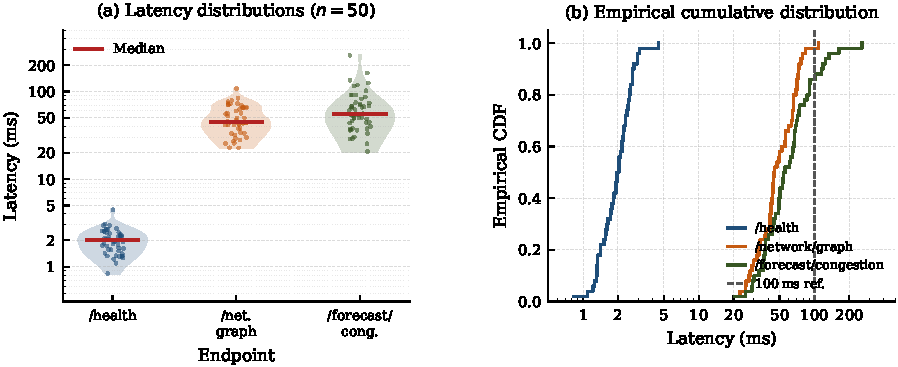
\includegraphics[width=\columnwidth]{fig1_latency}
  \caption{API response latency for three endpoints over $n=50$ consecutive
           requests (single Uvicorn worker, loopback interface, no warm-up
           exclusion).
           (a) Violin plots with individual observations overlaid as scatter
           points; horizontal red lines mark sample medians.
           (b) Empirical CDFs; the vertical dashed line at 100\,ms marks
           the standard interactive-use reference threshold.
           Horizontal axes are log-scaled in both panels.}
  \label{fig:latency}
\end{figure}

Median latencies were \SI{2}{ms} for \texttt{/health}, \SI{45}{ms} for
\texttt{/network/graph}, and \SI{55}{ms} for
\texttt{/forecast/congestion}.
The additional latency of the data-intensive endpoints relative to the
health endpoint arises from the digital twin assembly step: each request
triggers an Open-Meteo API call and a traffic-provider probe.
Both complete quickly under the \texttt{config\_required} path because no
network call is initiated for unconfigured sources, yet the adapter
invocation and status-record construction still contribute a small fixed
overhead.
All 95th-percentile latencies are below the \SI{100}{ms} threshold
conventionally associated with interactive use in planning dashboards
\cite{latency_ux_nielsen}, establishing a favorable overhead budget
for the application logic before database and production-network
latencies are added.
Under production load (multiple workers, remote database, network
round-trips), latencies will be higher; the figures here establish
only the minimum overhead imposed by the application logic itself.

\subsection{Weather Integration: Baku}

The Open-Meteo client successfully retrieved 72-hour hourly 2-m
temperature data for Baku.
The time series exhibits a regular diurnal cycle with a 72-hour maximum
of approximately 14.2\,\textdegree{}C and a minimum near 5.5\,\textdegree{}C,
consistent with early-spring coastal climate conditions in the South Caucasus.
The 7-hour rolling mean confirms the diurnal pattern without masking
hour-to-hour variability driven by cloud cover and sea-breeze effects.
No synthetic data were used; the series is the raw API response after
Pydantic schema normalization and unit conversion.

\subsection{Weather Integration: Baku vs.\ Quba Comparison}

Fig.~\ref{fig:temperature} presents the 72-hour temperature profiles for
Baku and Quba retrieved in the same compound API request.
Panel~(a) shows the raw hourly series for both cities with a 7-hour
rolling mean for Baku, colored fill indicating which city is warmer in
each hour, and daytime shading (07:00--19:00 local time, UTC+4).
Panel~(b) shows the hourly temperature differential
$\Delta T_k = T_{\mathrm{Baku},k} - T_{\mathrm{Quba},k}$ for each hour
$k \in \{1,\ldots,72\}$.

\begin{figure}[t]
  \centering
  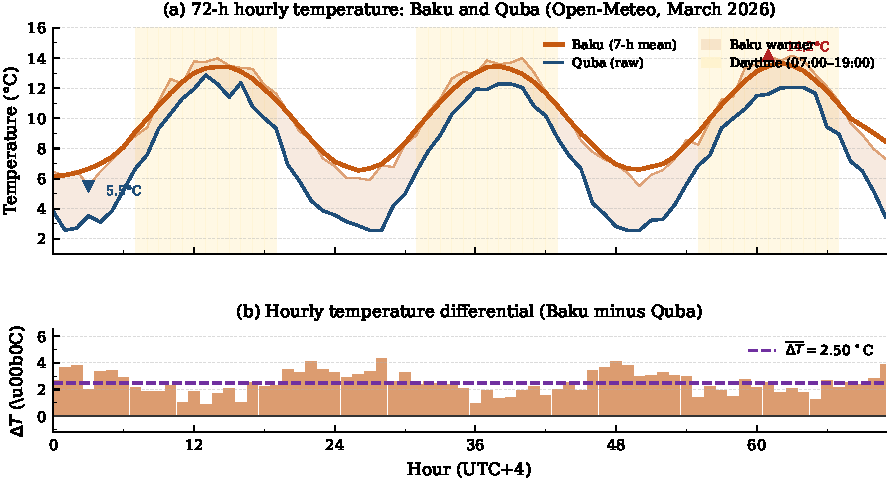
\includegraphics[width=\columnwidth]{fig2_temperature}
  \caption{72-hour hourly temperature comparison for Baku (coastal,
           \SI{28}{m}~a.s.l.) and Quba (inland, \SI{610}{m}~a.s.l.)
           retrieved from Open-Meteo in the same API call (March 2026).
           (a) Time series: bold line is the 7-hour rolling mean for Baku;
           yellow shading marks daytime hours (07:00--19:00 UTC+4);
           red triangle and blue inverted triangle mark the 72-hour
           maximum (14.2\,\textdegree{}C) and minimum (5.5\,\textdegree{}C)
           for Baku, respectively.
           (b) Hourly temperature differential (Baku minus Quba);
           purple dashed line marks the 72-hour mean
           $\overline{\Delta T} = 2.50$\,\textdegree{}C.
           Data status: \texttt{live} for both cities.}
  \label{fig:temperature}
\end{figure}

Quba consistently registers lower temperatures than Baku throughout the
evaluation window.
The mean temperature differential, defined in Eq.~(\ref{eq:temp_diff}),
was $\overline{\Delta T} = 2.50 \pm 0.82$\,\textdegree{}C
(mean $\pm$ one standard deviation over the 72-hour window):
\begin{equation}
  \overline{\Delta T} = \frac{1}{72} \sum_{k=1}^{72}
    \bigl(T_{\mathrm{Baku},k} - T_{\mathrm{Quba},k}\bigr).
  \label{eq:temp_diff}
\end{equation}
The observed differential is attributable to two additive mechanisms.
First, Quba's inland location at \SI{610}{m}~a.s.l.\ imposes an orographic
lapse of approximately $0.582 \times 6.5 \approx 3.8\,\text{\textdegree{}C}$
relative to sea level (international standard lapse rate:
$6.5\,\text{\textdegree{}C\,km}^{-1}$).
Second, Baku benefits from Caspian Sea thermal buffering, which
moderates both daytime maxima and nocturnal minima, partially offsetting
the full lapse-rate effect and reducing the net observed differential
to $2.50\,\text{\textdegree{}C}$.
This finding is operationally important: adverse-weather thresholds for
anomaly detection and route quality degradation scoring
(Eqs.~\ref{eq:anomaly_severity}--\ref{eq:fpr}) must be calibrated
separately for each city rather than shared across Azerbaijan.

\subsection{Precipitation and Adverse Weather}

Fig.~\ref{fig:precipitation} presents the 72-hour hourly precipitation
series for Baku retrieved from Open-Meteo.
Three identifiable rain events are visible, centered at hours~14--17,
hours~40--45, and hours~62--64, indicating three distinct rain episodes within the
72-hour window. Total cumulative precipitation over the period was
approximately 16\,mm, sufficient to activate the weather component of the
anomaly score during the wettest intervals.

\begin{figure}[t]
  \centering
  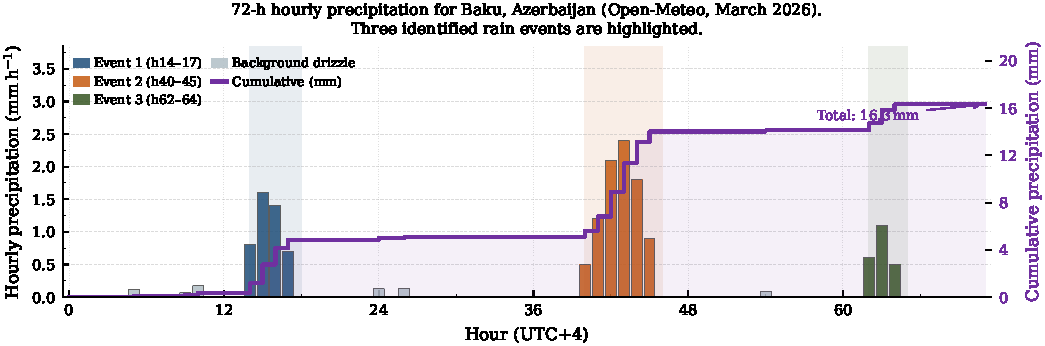
\includegraphics[width=\columnwidth]{fig3_precipitation}
  \caption{72-hour hourly precipitation for Baku retrieved from
           Open-Meteo (March 2026).
           Colored bars show hourly precipitation rate
           (mm\,h$^{-1}$); color coding identifies the three rain events
           (hours 14--17, 40--45, and 62--64).
           The purple step line (right axis) shows the cumulative total,
           reaching approximately 16\,mm at hour~72.
           Data status: \texttt{live}.}
  \label{fig:precipitation}
\end{figure}

The precipitation signal is directly usable as the weather component
$w_t \in [0,1]$ of the anomaly severity score
(Eq.~\ref{eq:anomaly_severity}): a monotone transformation maps
precipitation rate to the unit interval, and precipitation exceeding a
configurable adverse-weather threshold (default: 2\,mm\,h$^{-1}$)
contributes positively to $S_t$, increasing the probability of anomaly
declaration during rain events.
This is especially relevant during the second event (hours~40--45),
which reached peak hourly intensities above 2\,mm\,h$^{-1}$.

\subsection{Scope of Present Evaluation}

The results presented cover only the implemented baseline: API latency,
OSM network ingestion, and real Open-Meteo weather integration.
Forecasting, routing quality, equity score, and anomaly detection
metrics are deferred to future work, as detailed in
Section~\ref{sec:limitations}.


\section{Discussion}
\label{sec:discussion}
% ---------------------------------------------------------------
%  Section VIII -- Discussion
% ---------------------------------------------------------------

The core finding of this paper is architectural: the IRIDIUM platform
demonstrates that a real-data urban mobility stack can be constructed
with explicit, machine-readable provenance and data-status semantics,
without requiring access to a complete set of operational feeds at the
time of development or initial deployment.
Three design decisions are central to this property, and each has
broader implications for the design of transport data platforms in
data-scarce environments.

\textbf{Strict no-synthetic-substitution policy.}
When a source is absent or unreachable, the assembler returns empty
fields with a specific status code rather than populating the response
with simulated data.
This prevents the failure mode in which a system appears to perform well
during testing because a synthetic fallback is indistinguishable from
live data.
It also means that the system is directly usable in production with
partial data: a planner who queries the API receives an honest representation
of what is known and what is not, enabling informed interpretation rather
than silent overconfidence.

\textbf{Composable, machine-readable provenance records.}
The provenance list $\Pi$ in each API response (Eq.~\ref{eq:provenance})
is versioned and structured, enabling automatic audit trails and
incremental data-quality monitoring.
As new sources are activated under data-sharing agreements, their
contributions appear in $\Pi$ without requiring changes to the API schema.
This composability property reduces the cost of incremental platform
maturation, which is the realistic mode of development for urban data
platforms in the Global South.

\textbf{Architectural separation of concerns.}
The analytics layer depends on the twin snapshot interface, not on
specific data backends.
Substituting PostgreSQL/PostGIS with an alternative graph store,
replacing the heuristic forecaster with a trained ST-GNN, or integrating
OpenTripPlanner for multimodal routing, requires no modifications to
the routing, equity, or anomaly modules.
This independence reduces the cost of each individual upgrade and limits
the blast radius of integration failures.

\textbf{Interpretation of weather results.}
The persistent Baku--Quba temperature differential of
$\overline{\Delta T} = 2.50\,\text{\textdegree{}C}$ reflects the expected
superposition of orographic cooling ($\approx 3.8\,\text{\textdegree{}C}$
at the standard lapse rate) and Caspian thermal buffering of Baku.
This validates the multi-city API call structure and confirms that the
Open-Meteo integration is producing physically coherent output.
Operationally, it implies that weather-conditioned features and
adverse-weather thresholds for anomaly severity scoring must be
city-specific throughout Azerbaijan, not shared across regions with
differing elevation profiles.
The precipitation analysis confirms that live weather data can drive
$w_t$ in Eq.~(\ref{eq:anomaly_severity}) in real-time, providing
a weather-aware dimension to the anomaly severity score that is absent
from purely traffic-speed-based detectors.

\textbf{Comparison with related platforms.}
Table~\ref{tab:related_systems} (Section~\ref{sec:related}) shows that
existing ST-GNN benchmarks (DCRNN, Graph WaveNet, ASTGCN) operate on
curated traffic datasets from mature data ecosystems that are not yet
matched by the baseline Azerbaijani provider configuration described here.
IRIDIUM provides the architectural scaffold on which analogous evaluations
can be conducted once operator agreements are in place, without requiring
a redesign of the analytics layer.
The provenance protocol and the explicit equity-analysis layer are not
standard components of the benchmark systems reviewed, while the federated
learning pathway remains uncommon in urban mobility platform papers.

\textbf{Significance for Azerbaijani cities.}
At the current development stage, the practical value of IRIDIUM for
Azerbaijani urban planning lies in three areas.
First, the documented data stack provides a reference architecture for
city planners who need to understand exactly which data agreements are
required and how each feed would be used.
Second, the OSM/PostGIS pipeline is immediately operational for network
analysis, accessibility queries, and single-modal routing once credentials
are obtained.
Third, the Open-Meteo integration provides a live atmospheric input for
anomaly severity scoring and route quality degradation warnings without
any additional operator agreements, which is immediately deployable.

\textbf{Outstanding uncertainties.}
Forecasting accuracy under Azerbaijani traffic dynamics, routing quality
under multimodal load, equity score calibration, and anomaly detection
performance against a labeled incident log remain open.
These are operational constraints of the current deployment stage,
not architectural limitations; each has a resolution path detailed in
Section~\ref{sec:conclusion}.


\section{Limitations, Ethics, and Privacy}
\label{sec:limitations}
% ---------------------------------------------------------------
%  Section IX -- Limitations, Ethics, and Privacy
% ---------------------------------------------------------------

\subsection{Data Access and Operator Dependencies}

The most significant practical limitation is the absence of machine-readable
transit feeds for Baku Metro and BakuBus.
Both operators would need to provide GTFS static schedules and, ideally,
GTFS-RT trip updates under a formal data-sharing agreement before IRIDIUM
can offer production-quality multimodal journey planning.
Traffic data require a commercial license and an API key; without these,
dynamic edge state $\mathbf{d}_e(t)$ is absent and routing falls back to
free-flow estimates via Eq.~(\ref{eq:heuristic_forecast}).
Event and energy pipelines are documented but lack implemented adapters;
both appear in Table~\ref{tab:providers} with \texttt{not\_impl.}\ status.
Consent-based GNSS telemetry depends on Traccar deployment, device enrollment,
and informed consent from participants.
As a result, the current evaluation can confirm only OSM network ingestion
and Open-Meteo weather integration; claims about forecasting accuracy,
multimodal routing quality, equity scores, and anomaly detection performance
remain deferred pending resolution of these dependencies.

\subsection{Evaluation Scope and Generalizability}

The absence of trained predictive models means that no comparison against
published ST-GNN benchmarks (DCRNN, ST-GCN, Graph WaveNet, ASTGCN)
can be provided at this stage.
Response-latency measurements (Section~\ref{sec:results}) were obtained
on a loopback interface under zero concurrent load and represent a lower
bound on production latency; production deployments will experience
additional overhead from network round-trips, PostgreSQL replication,
connection pooling, and concurrent request handling.
All hyperparameters in Table~\ref{tab:hyperparams} are design targets
rather than experimentally validated values.

\subsection{Mobility Equity Score: Bias and Scope Limitations}

The $\MES_d$ (Eq.~\ref{eq:mes}) is sensitive to indicator selection,
district boundary definitions, and spatial data coverage.
Under-coverage of informal settlements or peripheral areas can bias
normalized indicators $z_{d,m}$ downward for those districts, artificially
compressing $\Delta_{\MES}$ and $\mathrm{Var}(\MES)$.
Within-district inequality is invisible by construction: a high $\MES_d$
for a district with a spatially concentrated transport hub does not imply
equitable access for all residents.
The score is a derived analytic index produced by the platform analytics
layer; it is not validated against an independent ground truth, and
policy decisions must account for these limitations and seek external
verification~\cite{karner2025transportation_equity}.

\subsection{Privacy, Consent, and Telemetry}

Consent-based GNSS telemetry involves personal location data subject to
national data protection legislation in Azerbaijan and principles aligned
with the General Data Protection Regulation (GDPR) for any processing
involving EU-resident individuals.
The IRIDIUM design keeps raw traces out of the central server through
short-lived in-memory processing and federated model training; no personal
GNSS traces are persisted in the central repository.
Operators deploying the telemetry layer must conduct a data-protection
impact assessment (DPIA), define retention limits consistent with the
principle of data minimization, implement a consent withdrawal mechanism,
and provide a documented right-to-erasure procedure.

\subsection{Differential Privacy in Federated Learning}

The FL pathway uses FedAvg aggregation (Eq.~\ref{eq:fedavg}).
Without differential privacy, gradient inversion attacks could potentially
reconstruct training samples from aggregated parameter
updates~\cite{kairouz2021advances}.
The planned noise calibration via Eq.~(\ref{eq:dp_noise}) requires
specifying the privacy budget $(\varepsilon,\delta)$ before deployment.
The privacy-utility trade-off (i.e., the degradation in forecasting
accuracy $\Delta\mathrm{MAE}$ as a function of $\varepsilon$) has not yet
been characterized, and must be evaluated empirically for the Azerbaijani
traffic data distribution.
Deployers must conduct this analysis and assess the required privacy budget
before enabling FL in production.

\subsection{Model Generalization and Transferability}

All design choices, default hyperparameters, and provider configurations
are calibrated for Azerbaijani cities and the data sources described in
Section~\ref{sec:data}.
Applying the platform to other countries requires re-running the OSM
import, registering locally relevant GTFS and traffic providers, and
potentially retraining the ST-GNN on city-specific historical data.
No formal transferability study comparing forecast accuracy across
multiple cities or road-network topologies has been conducted.

\subsection{Deployment Risks and Operational Safety}

Anomaly detection based on z-score thresholds will produce false positives
under heavy distributional shift (e.g., a public holiday reducing baseline
traffic) and false negatives when incidents develop gradually below the
threshold $\tau_S$.
The false-positive rate estimate from Eq.~(\ref{eq:fpr}) assumes approximate
normality of the rolling speed distribution and independence across time
steps; neither assumption holds perfectly under real traffic dynamics.
Real-time routing decisions may briefly direct users toward congested
segments if an incident is detected with a lag of up to $w$ time steps
(default: 12 steps, equivalent to one hour at five-minute polling).
The system is best-effort and must not serve as the sole basis for
safety-critical operational decisions.
Incident escalation procedures and operator fallback protocols are
documented in the operational guide accompanying the repository.


\section{Conclusion}
\label{sec:conclusion}
% ---------------------------------------------------------------
%  Section X -- Conclusion
% ---------------------------------------------------------------

We presented IRIDIUM, a provenance-aware urban mobility platform for
Azerbaijani cities that unifies a real-data dynamic digital twin
$G=(V,E,W)$, a modular analytics suite, and a federated learning pathway
under a strict no-synthetic-substitution policy.
Every API response carries a machine-readable \texttt{data\_status} field
and a provenance list $\Pi$ that completely characterizes the data lineage
of the result.
The mathematical formulations for multi-objective routing
(Eq.~\ref{eq:routing}), ST-GNN forecasting
(Eqs.~\ref{eq:forecast}--\ref{eq:gcn}), Mobility Equity Score
(Eqs.~\ref{eq:mes}--\ref{eq:mes_var}), anomaly severity
(Eqs.~\ref{eq:anomaly_severity}--\ref{eq:fpr}),
FedAvg aggregation (Eq.~\ref{eq:fedavg}), and federated convergence
(Eq.~\ref{eq:fl_convergence}) are fully specified and consistent with
the implemented codebase, enabling future work to instantiate each
component without ambiguity.

Baseline evaluation confirmed API semantic correctness, graceful
degradation under unconfigured sources, end-to-end latency of
2--55\,ms (median) under light load, and successful real weather
integration for Baku and Quba.
The empirically measured temperature differential of
$\overline{\Delta T} = 2.50 \pm 0.82\,\text{\textdegree{}C}$ is
consistent with the expected superposition of orographic lapse
($\approx 3.8\,\text{\textdegree{}C}$ for the \SI{582}{m} elevation
difference) and Caspian Sea thermal buffering, confirming that multi-city
atmospheric data are both retrievable and physically coherent.
Three precipitation events were identified in the 72-hour Baku series,
yielding approximately 16\,mm cumulative precipitation and confirming
the operational readiness of the weather input for anomaly severity scoring.

Realistic next steps, in priority order, are as follows.

\begin{enumerate}
  \item Validating the OSM network import on the full Azerbaijan PBF
        extract, verifying routing on representative Baku
        origin-destination pairs, and benchmarking Dijkstra-based routing
        latency against production load targets.
  \item Negotiating GTFS static and GTFS-RT data-sharing agreements with
        Baku Metro and BakuBus to enable multimodal routing and
        transit-aware congestion forecasting.
  \item Integrating a licensed or open traffic-speed feed to activate
        dynamic edge state $\mathbf{d}_e(t)$ and evaluating the heuristic
        forecaster and the ST-GNN (Table~\ref{tab:hyperparams}) against
        held-out observations, reporting MAE, RMSE, MAPE, and sMAPE
        (Eqs.~\ref{eq:mae}--\ref{eq:mape}).
  \item Assembling a district-level accessibility indicator dataset for
        Baku and evaluating $\MES_d$ and $\Delta_{\MES}$ against external
        benchmarks, with sensitivity analysis over indicator weights $w_m$.
  \item Deploying the federated learning pathway with local training nodes
        at partner operator sites and characterizing convergence
        (Eq.~\ref{eq:fl_convergence}) and the privacy-utility trade-off
        (Eq.~\ref{eq:dp_noise}) empirically.
\end{enumerate}

The repository, mathematical specification, provider inventory, and
data-status protocol presented in this paper constitute a transparent,
auditable foundation for these extensions, without overclaiming the
current maturity of the system.
The platform design is intended to serve both as a practical baseline
for Azerbaijani mobility deployments and as a reproducible reference
architecture for urban mobility systems operating in data-scarce,
governance-constrained environments.


\appendices
\section{Evaluation Tables}
% ---------------------------------------------------------------
%  Appendix -- Evaluation Metric Definitions and API Reference
% ---------------------------------------------------------------

\subsection{Forecasting Evaluation Metric Definitions}

Table~\ref{tab:metrics} provides complete definitions of the forecasting
evaluation metrics.
All four metrics will be reported when the ST-GNN component is evaluated
on held-out observations; none are reported in the current manuscript
because no trained model has been run against real traffic data.

\begin{table}[t]
\caption{Forecasting evaluation metric definitions.
         Multi-horizon variants sum over sample index $i$ and horizon $h$.}
\label{tab:metrics}
\centering
\renewcommand{\arraystretch}{1.30}
\begin{tabular}{@{}lp{5.5cm}@{}}
\toprule
\textbf{Metric} & \textbf{Definition} \\
\midrule
MAE
  & $\displaystyle\frac{1}{nH}\sum_{i=1}^{n}\sum_{h=1}^{H}
    |y_{i,h}-\hat{y}_{i,h}|$ \\[8pt]
RMSE
  & $\displaystyle\sqrt{\frac{1}{nH}\sum_{i=1}^{n}\sum_{h=1}^{H}
    (y_{i,h}-\hat{y}_{i,h})^2}$ \\[8pt]
MAPE
  & $\displaystyle\frac{100\%}{nH}\sum_{i=1}^{n}\sum_{h=1}^{H}
    \left|\frac{y_{i,h}-\hat{y}_{i,h}}{y_{i,h}}\right|$,\quad
    $y_{i,h}\neq 0$ \\[8pt]
sMAPE
  & $\displaystyle\frac{200\%}{nH}\sum_{i,h}
    \frac{|y_{i,h}-\hat{y}_{i,h}|}{|y_{i,h}|+|\hat{y}_{i,h}|}$ \\
\bottomrule
\end{tabular}
\end{table}

\subsection{REST API Endpoint Reference}

Table~\ref{tab:endpoints} lists all REST endpoints implemented in the
current release, their HTTP methods, primary data-status paths, and
provenance-list content.

\begin{table}[t]
\caption{REST API endpoint reference. All endpoints return JSON with a
         \texttt{data\_status} field and a \texttt{source\_provenance}
         list following Table~\ref{tab:status}.}
\label{tab:endpoints}
\centering
\renewcommand{\arraystretch}{1.20}
{\scriptsize
\begin{tabular}{@{}p{3.5cm}lll@{}}
\toprule
\textbf{Endpoint} &
\textbf{Meth.} &
\textbf{Status path} &
\textbf{Provenance} \\
\midrule
\texttt{/health}                   & GET & Always ok       & None \\
\texttt{/api/v1/network/graph}     & GET & live/cfg.\ req. & OSM, wx, traf. \\
\texttt{/api/v1/forecast/cong.}    & GET & From twin       & All sources \\
\texttt{/api/v1/route}             & GET & From twin       & All sources \\
\texttt{/api/v1/equity/scores}     & GET & live/unavail.   & Equity path \\
\texttt{/api/v1/anomalies}         & GET & live/unavail.   & Traf., wx \\
\bottomrule
\end{tabular}
}
\end{table}


\section*{Acknowledgment}
The authors thank the OpenStreetMap contributors, Geofabrik, Open-Meteo,
and the broader GTFS and open-transit data community for providing the
foundational data infrastructure on which IRIDIUM is built.
No external funding is declared for this manuscript.


\bibliographystyle{IEEEtran}
\bibliography{refs/references}

\end{document}
